\subsection{Selection}
\label{sec:background:genetic_programming:selection}
  The selection process in GP is similar to that of GAs.
  However, unique modifications have been proposed for the standard process in 
  GP, which consider the semantics, or the functional behavior, of the programs 
  being evolved~\autocite{liskowskiComparisonSemanticawareSelection2015}.
  This work will not delve into this topic, as it is beyond the scope of this
  document.

  For the problem under study, we use a selection process similar to the one 
  used in the \textit{One Max} problem (a simple optimization problem where the 
  objective is to maximize the number of ones in a binary string).
  The equation for calculating the selection probability will diverge from 
  \vref{eq:selection_probability}, as it presumes the fittest individual is the 
  one with the highest fitness value.
  In contrast, the symbolic regression problem, which is our focus, considers the
  individual with the lowest fitness value as the fittest.

  For this particular case of the symbolic regression problem, we adjust our 
  approach to selection.
  We introduce a \emph{corrected fitness function}, \(\phi'\), defined as:

  \begin{equation}
    \label{eq:bg:gp:sym:corrected_fitness}
    \phi'(I) = \left(\sum \Phi_\mathbf{P}\right) - \phi_I
  \end{equation}

  Here, \(\phi_I\) signifies the fitness of individual \(I\), and 
  \(\Phi_\mathbf{P}\) represents the \textit{batch fitness function} defined in 
  \vref{def:batch_fitness_function} applied to the population \(\mathbf{P}\).
  We then define the selection probability for an individual \(\mathbf{P}_i\) as:

  \begin{equation}
    \label{eq:bg:gp:sym:selection_probability}
    p_i = \frac{\phi'(\mathbf{P}_i)}{\sum_{j = 1}^N \phi'(\mathbf{P}_j)}
  \end{equation}

  In this equation, \(N\) stands for the size of the population.

  With this methodology, we calculate the selection probabilities for the 
  population as illustrated in \vref{tab:bg:gp:sel:prob}.
  The outcome shows that 
  the individual with the highest error has a considerably low probability of 
  being selected, while the other individuals have roughly equal chances.

  \subimport{.}{tab-bg-gp-sel-prob.tex}

  Assuming a \emph{survival rate} of 50\%, let's consider that the selection
  process favors \(I_2\) and \(I_3\) as survivors due to their higher selection
  probabilities (as shown in the previous table).
  In this scenario, \(I_1\) and \(I_4\) are identified as the ones to be replaced
  by the offspring in the next generation.
  A comparison between the survivors and the target function is shown in
  \vref{fig:bg:gp:sel:prob}.

  \begin{figure}[ht!]
    \centering
    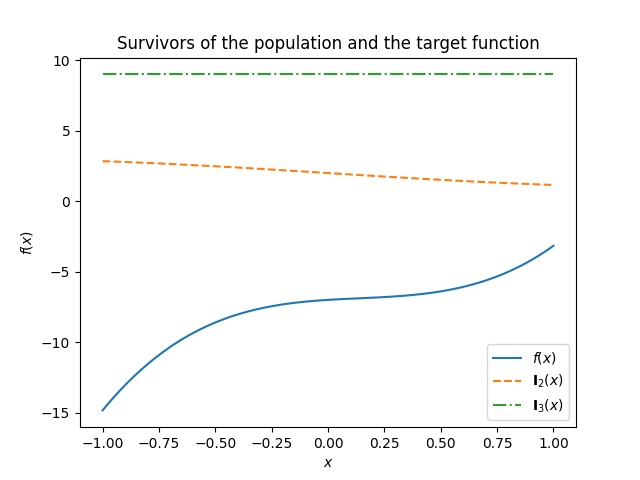
\includegraphics[width=0.6\textwidth]{img/theoretical_framework/gp_pop_sel_survivors.png}
    \caption{Comparison between the survivors and the target function.}
    \label{fig:bg:gp:sel:prob}
  \end{figure}

  Selection remains a cornerstone of evolutionary algorithms, ensuring that 
  individuals possessing beneficial traits have a greater likelihood of 
  transferring those traits to subsequent generations. While nuances 
  distinguish the selection processes of Genetic Programming (GP) and Genetic 
  Algorithms (GAs), the underlying principle remains: to direct the search 
  towards more promising regions of the solution space. As we progress further, 
  it's essential to recognize the interplay between selection and other 
  operators, understanding that their combined effects mold the trajectory of 
  the evolutionary process. The insights gleaned from this understanding will 
  aid in fine-tuning algorithms and achieving better results in future 
  endeavors.
